\documentclass[a4paper, 12pt]{article}

\usepackage{amsmath}
\usepackage{graphicx}
\usepackage{float}

\begin{document}
	
	\pagenumbering{arabic}
	\title{Surface Area of Spheres - the Wok Problem}
		\author{Nick Wang}
		\date{\today}
	\maketitle
	
	\section{Introduction}
	\paragraph
		\indent Since the first introduction to geometry in elementary school, students have investigated the volume, surface area, and many other geometric properties of 2-Dimensional,as well as 3-Dimensional shapes. Yet one area students do not intuitively understand is circles and spheres, especially the derivation of area formula, volume area, etc. As a part of the curriculum of second year Calculus course, today we look at one of these problems and approach from a Calculus point of view:\\
		\begin{center}
			\textit {One such problem states that a semi-spherical wok exists with diameter of 16 cm and height 9 cm. We are to paint the outside and inside of 5000 woks with 0.5 mm thick of paint each. Calculate the volume of paint needed in liters. }\\
		\end{center}
		\begin{figure}[h]
			\label{wok dimensions}
			\centering
			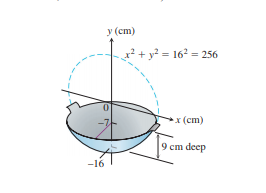
\includegraphics[width=0.5\textwidth]{wok.png}
			\caption{Wok Dimensions}
		\end{figure}
	
	\section{Interpolation}
	\paragraph
		\indent The problem states that a wok needs to be painted on both its inside and outside. This meant the area to paint is the surface area of the wok's inside and outside. Additionally the paint is painted 0.5 mm thick, which meant the volume of paint needed on each side is the surface area multiplied by the height of the paint, which is 0.5 mm. This meant the  real question this question is asking is what is the surface area of part of a sphere, since height is known.\\\\
		\indent Realizing this we can use the formula $A = \int2\pi y\sqrt{1^2+\frac{dy}{dx})^2}dx$ to calculate surface area This indeed meant the calculation must be done in terms of $dx$, which will be addressed.\\\\
		\indent Thus we need to find $f'(x)$ with given equation $$x^2+y^2=256$$\\
		\indent Furthermore since the wok represents part of a sphere. And a sphere can be represented by rotating a function representing a semicircle around the x axis, if the function is in terms of $x$.To rewrite the equation of the entire circle as a function of $x$. Simplifying we get:$$y=\sqrt{256-x^2}$$\\
		\indent This equation does not match the diagram shown in the given graph, it is the rotation of the diagram. This satisfied the condition that the function is in terms of $dx$.
		\begin{figure}[H]
			\label{Wok-2d}
			\centering
			\includegraphics[width=0.3\textwidth]{wok-2d.png}
			\caption{Equation of the wok}
		\end{figure}
		\indent The wok is imagined to be lying between the first and fourth  quadrant from $x=7$ to $x=16$. Thus only half of the wok is visible on the graph. This also meant o a full rotation  contains the entire surface area of the sphere  without overlapping.
		\indent Using equations we got previously: $$\frac{dy}{dx}=\frac{1}{2}{(256-x^2)}^{-1/2} 2x$$
		We can now plug in the equation and the bounds from $x=7$ to $x=16$:$$A = \int_7^{16} 2\pi \sqrt{256-x^2}\sqrt{1^2+{(\frac{1}{2}{(256-x^2)}^{-1/2} 2x)}^2}dx$$
		\indent Simplifying each term inside the integral:$$A =2\pi \int_7^{16} \sqrt{256-x^2}\sqrt{1+{(256-x^2)}^{-1} x^2}dx$$
		\indent Changing negative exponent to a fraction:$$A =2\pi \int_7^{16} \sqrt{256-x^2}\sqrt{1+\frac{x^2}{256-x^2}}dx$$
		\indent Rewriting 1 with common denominator $256-x^2$:$$A =2\pi \int_7^{16} \sqrt{256-x^2}\sqrt{\frac{256-x^2}{256-x^2}+\frac{x^2}{256-x^2}}dx$$
		\indent Combining terms with common denominator: $256-x^2$:$$A =2\pi \int_7^{16} \sqrt{256-x^2}\sqrt{\frac{256-x^2 + x^2}{256-x^2}}dx$$
		\indent Canceling out similar terms and pulling out constant 256:$$A =2\pi \int_7^{16} \sqrt{256-x^2}16 \sqrt{\frac{1}{256-x^2}}dx$$
		\indent Moving the constants out of the integral and simplifying the integrand:$$A =32\pi \int_7^{16}{(256-x^2)}^{1/2} {(256-x^2)}^{-1/2}dx$$
		\indent Combining similar terms by adding up the coefficient:$$A =32\pi \int_7^{16}{(256-x^2)}^{1/2-1/2} dx$$
		\indent Simplifying the integrand, a function to the 0 power is 1:$$A =32\pi \int_7^{16}1 dx$$
		\indent Taking the integral:$$A =32\pi \left[x\right]_7^{16}$$
		\indent Plugging in the bounds:$$A =32\pi {(16-7)}=288\pi$$
		\indent Thus we have found the surface area of one side of the wok in $cm^2$. To calculate the total volume of paint needed, we multiply the surface area. In order to convert final result to liters, we use dimensional analysis:$$V=\frac{288\pi cm^2}{1 side}\cdot\frac{ 0.5 mm}{1 side} \cdot\frac{1 cm}{10 mm}\cdot\frac{1 side}{1 wok}\cdot5000 wok\cdot\frac{1 liter}{1000cm^3}=72\pi/side$$\\
		\indent Thus to paint 5000 woks of this dimension we need $72\pi$ liters of paint for each side of the wok.

	\section{Conclusion}
	\paragraph
		\indent This problem investigates the properties of surface areas of spheres by connecting them to real life situations. The problem is complicated by hiding under what seems to be a volume problem. At first glance it seems that this is a washer or a intersection. Placing the sphere below the x axis and perpendicular to the y axis it first sets up the problem in a uncomfortable position, but with some analysis it can be determined that rotating the sphere on top of the x axis will greatly simplify the calculation without changing the result. During the calculation we investigated the properties of a sphere without using any specific equation and derived at the result that 5000 woks would require $72\pi$ liters of paint. The similar  process can be used on a general case to derive the formula of the surface area of spheres  for further investigation.

\end{document}